\section{Background}

Boeing was founded on July 15, 1916 by William Boeing and is the world's leading aerospace company\footnote{The Boeing Company: \url{http://www.boeing.com/}}. %\todo{(Boeing, 2016)}. 
This study took place in one of their subsidiary companies called Jeppesen founded in 1934\footnote{Jeppesen - Transforming the Way the World Moves: \url{http://ww1.jeppesen.com/index.jsp}}. They offer a diverse set of products such as navigation charts, planning tools and crew management systems. This study focuses on the last. In this section we discuss the background of the company, presenting an overview of their crew management systems, the interfaces we studied and the avocado model.

%VALE PRWTA TO CREW MANAGEMENT SYSTEMS
\subsection{Crew management systems}

An enormous amount of airlines expenses comes from the costs of moving crew. Jeppense's office in Gothenburg specialises in providing crew management solutions to airlines so as to increase the crew productivity. The planning process is very complex and consists of a number of different stages:

\begin{itemize}
\item {\em Manpower process}: %the general number of crew members, along with the required qualifications is defined. This can be considered as defining 
anonymous work-blocks for crew personnel are defined together with required qualifications. These work-blocks %where they 
should be filled by real people later on and the companies can decide who should be hired, promoted, who needs training and how the leave should be divided.
\item {\em Pairing:} set of flight legs, which start and end in the same destination. This is a sophisticated process where a large number of factors should be taken into consideration.  When the crew comes back, the pairing is finished. 
There are a lot of restrictions such as the hours the crew can work, how many continuous days they are allowed to work, the different workforce laws of the country they come from to name a few. 
\item {\em Rostering:} 
%The next process is called rostering and it is about 
assigning actual personnel so to define the %. The rosters can be viewed as the 
actual work schedules. Again, here there are lot of restrictions. For example, a trip going to Brazil requires at least one crew personnel who can speak Portuguese. What is more, a crew member might wish to take a few days off and therefore another crew member should replace him or her for. Sometimes crew cannot work together or they should work together. 
\item {\em Crew tracking stage:}
%Finally, there is the crew tracking stage. This is where 
the company tries to solve problems when they arise. For example, a crew member who got sick in the middle of his or her assigned trip has to be replaced by another member who is on standby in this city.  
\end{itemize}

Valid and consistent information exchange between different systems is crucial for the optimization system to provide the best results. However different airlines have different customization needs. Consequently, their systems vary with each other. This imposes a threat for the information interoperability as there is a risk for misinterpretations of the exchanged data.  



\subsection{Standard interfaces }

International Air Transport Association (IATA)~\cite{IATA} provides support for most airline companies throughout the world. The IATA manual defines the structure and behaviour of both interfaces of the study. We used the issue of March 2011 for the study. 


\subsubsection{SSIM interface}
The Standard Schedules Information Manual (SSIM) defines the interface which is complied to the IATA regulations. It is used from airline companies to produce schedule data in the form of timetable information. The airline companies generate an SSIM file which is then distributed to multiple recipients such as airline reservation systems, timetable agencies, air traffic control authorities and so on~\cite{IATA}.
Jeppesen systems use these files for crew and fleet management, with a strong emphasis on optimization of crew pairing, rostering and tracking. The need for the consistency of the data is therefore considered highly important in order to create valid and efficient solutions.



The interface under investigation has been selected because it is  well-known by the people in the company and it is well-defined by the IATA manual. However it contains a number of variability points. This means, there are parts of the standard which are open for interpretation that the interface should be aware of. Therefore, it was considered a good candidate to provide a basis for this research, where the outcome could be replicated to other similar interfaces as well. 

The manual provides explicit formatting rules to define the interface's syntax. Each byte in the syntax has its own meaning and corresponds to one of the supported fields. It should be noted that the company's systems do not read all the fields, since some of the optional fields such as meal service, have no impact on crew planning and are therefore discarded.


\subsubsection{Operational messages interface}

The second interface is about the operational messages, which could be considered as a family of formats. They are concerned with information regarding amendments of flight schedules, deviations from original schedules and aircraft movements. 
The information are being exchanged between airlines, aircraft and schedule aggregators~\cite{IATA}. % (International Air Transport Association, 2011). 


An identifier is placed at the beginning of the message to differentiate between each format. Information for permanent changes to basic schedules are transmitted through the Standard Schedules Message (SSM). Modifications of schedules are defined through the Ad-Hoc Schedules Message (ASM). Aircraft Movement Messages (MVT) are concerned with messages regarding departure, arrival and delay of a flight which were produced manually. Aircraft Initiated Movement Message (MVA) are concerned with messages of the same nature as with MVT but produced by the aircraft itself~\cite{IATA}. % (International Air Transport Association, 2011).


The manual provides guidelines for specifying a diverse set of actions for each of these formats, in the form of sub-messages. These actions, for example, can define behaviour for inserting a new flight designator, update information of existing flights and change of existing routing information. Each of these sub-messages are specified in a similar fashion as with the SSIM's case; each byte corresponds to a field which contain data for messages between the aircraft and the airport. Not all the messages are being used by each airline. 

\subsection{The old and the new system}
In this section we present the difference between the old and the new system for when it comes to parse SSIM files. 

\subsubsection{The old system}
The variability binding takes different approaches in the two systems. The old system provides a form that allows its users to define many parameters when they wish to import the raw data from SSIM files, giving them the capability to configure the system in run time. These parameters correspond to one more flags of the tool. Some of them are taken from the input form, some are taken from the configuration files. The files are then converted to a specified format and handled by the same component of the tool.

The original code, which was written in C language, was closely following the IATA format and it was expected to be used in the same way by all the customers. In reality, the algorithms had to be adjusted to accommodate more customer specific requirements. 
%This resulted in an immense main function, with many global variables, that is extremely complex, 
This resulted in an extremely complex code which was 
hard to read and manage, as described by the company's experts. Although it works correct and satisfies the expected functional requirements, it is hard to maintain as there is a high risk of problems occurring when the system is updated.

\subsubsection{The new system}
The new system divides the work of interpretation and logic handling between the adaptor and the back end, as shown in Figure~\ref{fig:newSystem}.  

\begin{figure}[h]
\centering
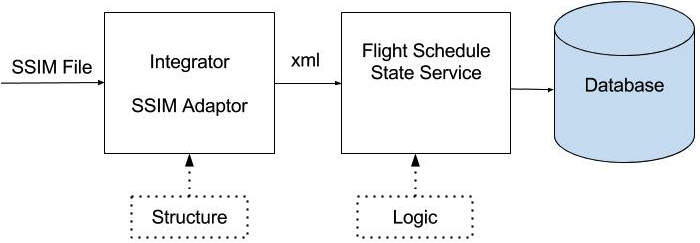
\includegraphics[width=\columnwidth]{figure/Figure2.png}

\caption{ General overview of parsing an SSIM file and storing it in the database}
\label{fig:newSystem}
\end{figure}


The aim is to have separation of concerns between these two components. The SSIM file is generated by an airline company and used as an input to the integrator. The integrator, consecutively, uses an adaptor to define the structure for the SSIM standard in XML form. The ``Flight Schedule State Service" component imports this XML file and applies some well defined computations to handle the given semantics accordingly. Finally it stores in the database the converted information. 

The integrator's code of the new system is wrote in Python. 
%was originally written in Java. However, during our analysis phase, the company changed the programming language to Python. Although the logic stayed somewhat the same, we had to perform additional code analysis and change our documentation appropriately. For example, the class diagrams had to be redrawn. Based on these diagrams we later placed our proposed solution. 
%An important aspect of our decision making was, for each variability point, which of these two components had to be selected. Whether or not it was a structural or logical problem. 
%Finally, it should be mentioned that the 
Within the old system variability is managed at run-time while in the new system the variability is bound at build-time. This means, the old system allows the users to change the interpretation of the parsing of SSIM files by providing an input form containing a number of parameters. However, the new system was initially designed and built to manage customer specific use cases. Later, when they changed the technology from Java to Python, they still provided plug-in scripts which extent the system's core architecture that address customer specific issues. 

%\subsection{The avocado model}
%The Avocado model demonstrates how the company develops its products. This Avocado Model is shown in Figure~\ref{fig:avocadoModel}.
%
%\begin{figure}[h]
%\centering
%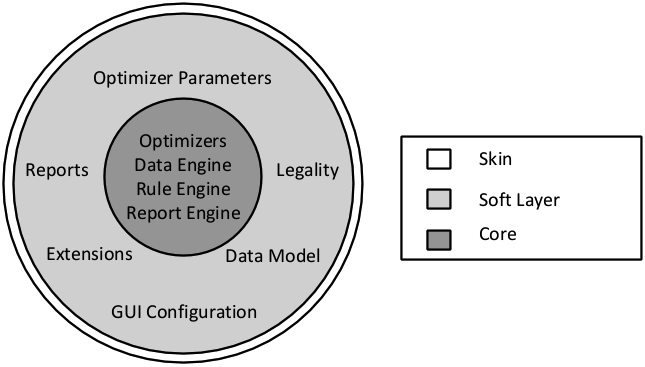
\includegraphics[width=\columnwidth]{figure/figure11.png}
%\caption{ The Avocado model. }
%\label{fig:avocadoModel}
%\end{figure}
%
%
%The core part consists of functionality that is the same to all of their customers. For example, all the optimization algorithms are embedded in the core. The translation of SSIM information to semantics is also inside the system's core. \\
%Then, there is the soft layer that surrounds the core. This layer contains the business logic and it can be different from customer to customer. For example, union contracts are different between the United States and Europe. Another example is how the graphical user interface is displayed from customer to customer. Even the translation of the SSIM can be modified to adhere to an airline's needs.
%This layer can be modified by the airlines companies alone, or with the help of Jeppesen engineers. The configuration can be done by utilizing a domain specific language developed by the company as well as by writing Python scripts which do not require the system to be recompiled. The soft layer therefore varies for each airline. Jeppesen does not have control over this layer after their system is delivered. It is up to the airlines to maintain it. \\
%Finally, there is the skin, which is the outer layer of the avocado. This is where the system allows its users to define parameters. For example, how many days off in a month can a crew member have. 








